\chapter{K-band (18-27.5~GHz) Focal Plane Array (KFPA)}\label{chap:kfpa}

\vspace{-0.5cm}
The K-band Focal Plane Array has seven beams total, each with dual circular
polarization.  Each beam covers the 18-27.5 GHz frequency range with fixed
separations on the sky with nominal offsets listed in
Table~\ref{table:kfpa_beam_offsets}.  The feeds have cooled polarizers
producing circular polarization.  The only internal switching mode is frequency
switching.  The seven feeds are laid out in a hexagon with one central feed as
shown in Figure~\ref{fig:kfpaFeeds}.  The hexagon is oriented such that the central
feed is not at the same cross-elevation or the same elevation as any of the
other beams.  Beam pairs (3,7) and (4,6) are at equal elevations and are
appropriate choices for nodding and peak/focus observations.

Unlike other receivers, the \gls{KFPA} uses variable noise diodes for each
beam (${\sim}10\%$ of the system temperature) that can change, so it is very
important for observers to calibrate their data every session.  The
maximum instantaneous bandwidth for the receiver is currently 1.8~GHz. An
experimental \dq{broadband} mode allowing 7.5~GHz of instantaneous bandwidth
is also available for single beam observations using either beam 1 or 2.

\noindent
\begin{minipage}[c]{0.65\linewidth}
\begin{center}
\vspace{0pt}
\captionof{figure}[Orientation of the KFPA feeds on the GBT]
{Orientation of the \gls{KFPA} feeds on the \gls{GBT}}
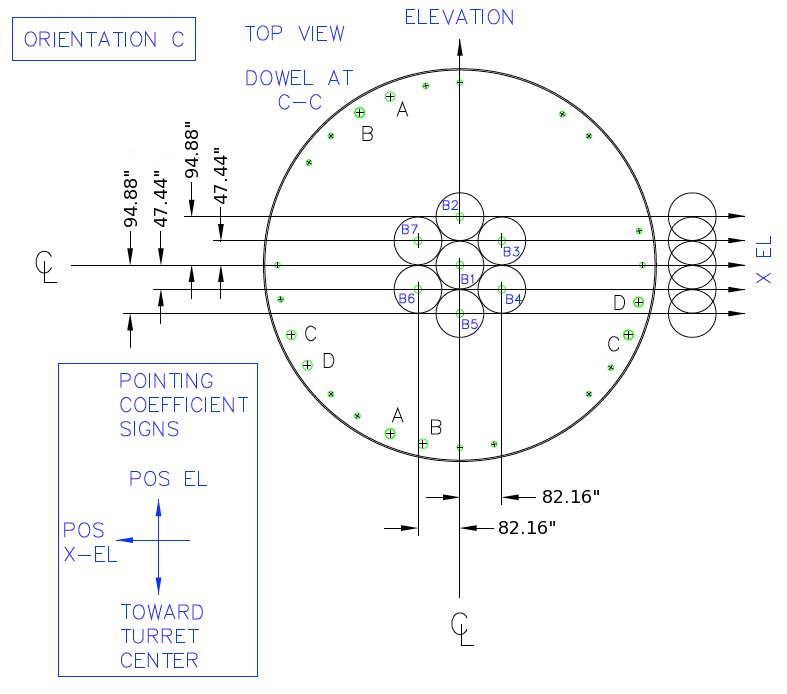
\includegraphics[width=\linewidth]{kfpaOrientC.jpg}
\label{fig:kfpaFeeds}
\end{center}
\end{minipage}
\hfill
\begin{minipage}[c]{0.35\linewidth}
\begin{center}
\vspace{0pt}
\begin{tabular}[b]{l d d}
\toprule
Beam & \multicolumn{1}{c}{$\Delta$X-El (\arcsecond)} &
\multicolumn{1}{c}{$\Delta$El (\arcsecond)} \\ \midrule
1  &    0.00 &   0.00 \\
2  &    0.00 &  94.88 \\
3  &  -82.16 &  47.44 \\
4  &  -82.16 & -47.44 \\
5  &    0.00 & -94.88 \\
6  &   82.16 & -47.44 \\
7  &   82.16 &  47.44 \\ \bottomrule
\end{tabular}
\captionof{table}[Nominal beam offsets of the KFPA]
{Nominal beam offsets for each feed of the \gls{KFPA}
at orientation C.}
\label{table:kfpa_beam_offsets}
\end{center}
\end{minipage}

\newpage

\section{Configuration}\label{sec:kfpa_configuration}

\subsection{Beam selection with VEGAS banks}
Observers can use all 7 \gls{KFPA} beams simultaneously, or select a only subset of
them. To maximize versatility and observing efficiency when mapping, most observers will
want to use the full set of 7 beams paired with the observations with the VEGAS backend.

An equal number of beams must be routed to Converter Rack Modules A and B, imposing the
following constraints on mapping beams to \gls{VEGAS} banks:

\begin{itemize}[leftmargin=*,itemsep=1pt]
\item A single beam may be routed to any  or all of the \gls{VEGAS} banks A$\rightarrow$H.
\item Dual-beam configurations allow each beam to be routed to a maximum of
4 \gls{VEGAS} banks.
\item When using 3--4 beams, each beam may be routed to up to a maximum of
2 \gls{VEGAS} banks.
\item When using more than 5 beams, each beam may only be routed to a
single \gls{VEGAS} bank.
\item When using all 7 beams, each beam may be routed to a single \gls{VEGAS} bank
with an optional second copy of beam 1 being routed to the remaining \gls{VEGAS}
bank. This is known as the \dq{7+1} mode of the \gls{KFPA}.
\end{itemize}

An example configuring for the 7+1 mode of the \gls{KFPA} is given in Script~\ref{lst:kfpaconfig}.

\subsection{Instantaneous Bandwidth}

\begin{itemize}[leftmargin=*]
\item {\bf Narrowband mode} is the default setting and must be used with any
\gls{KFPA} multi-beam configuration. In this mode all frequencies must have a
maximum frequency separation of 1.8~GHz and lie within 900~MHz of the doppler
tracking frequency.

\item {\bf Broadband mode} mode allows the system to process up to 7.5~GHz of
bandwidth. This mode is only available for single beam observations using either
beam 1 or beam 2 and is acheived by setting {\tt broadband=1} in the
configuration (see \S~\ref{sec:keywords}).
\end{itemize}


\section{Calibration}

The \gls{KFPA} receiver has variable noise-diodes that can change so it is
important that users calibrate their data for every session.  The diodes have
effective temperatures that can drift slowly over time or change after a thermal
cycle of the cyrostat.

We currently recommend that users calibrate their data by carrying out
{\bfseries{\textcolor{pythonKeywords}{Nod\textnormal{/}OnOff}}} observations
on a known flux calibrator using the same configuration that they would
use for their science observations.  An example \gls{SB} for performing this
type of calibration using all 7 beams of the \gls{KFPA} is shown in
Script~\ref{lst:kfpa_calibration}.

It is also possible to use the sky at different elevations to \dq{flat-field}
the relative gains of the beams and then absolute calibrate the data with an
{\bfseries{\textcolor{pythonKeywords}{OnOff\textnormal{/}Nod}}}
observation of one reference beam using a known flux calibrator.
Calibration using resolved sources such as planets or the Moon adds
the requirement for an accurate temperature model of the source plus a
model for coupling the GBT beam to the planet disk.  Observers wishing to
use such methods should consult the \dq{Friend} of their project to devise the
best strategy for calibration.

\newpage

\lstinputlisting[language=PythonAstrid,
backgroundcolor=\color{sbBackground},
caption={[KFPA calibration SB.]
An example \gls{SB} used to calibrate \gls{KFPA} noise diodes for all 7 beams.},
label={lst:kfpa_calibration}]
{kfpa_calibration.py}

\subsection{Realigning the Noise Diodes}

Sometimes the effective temperature of the noise diodes can suddenly change by
signficant amounts due to firmware configuration glitches that may occur after
reseting the manager, updates to receiver parameters, and power failures.
A large change the effective temperature of a noise diode could result in unusual
$T_{sys}$ values or a large difference between the amplitude of beams in azimuth
Peak scans as shown in Figure~\ref{fig:kfpa_bad_cals}.

\vspace{-0.25cm}

\begin{figure}[!h]
\begin{center}
\subfloat[KFPA azimuth pointing scan where noise diode
temperatures have drifted.  The amplitude of beam 3 is approximately
3 times that of beam 7.\label{fig:kfpa_bad_cals}]
{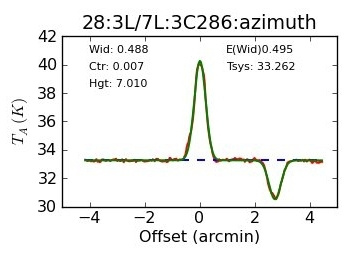
\includegraphics[width=.475\linewidth]{kfpa_bad_cals.jpg}}
\hfill
\subfloat[KFPA azimuth pointing scan after realigning the noise diodes.
Beam amplitudes are approximately equal.\label{fig:kfpa_good_cals}]
{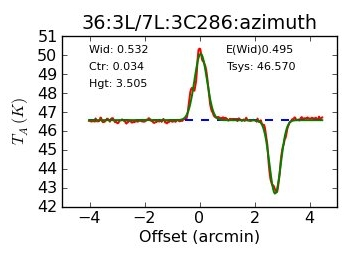
\includegraphics[width=.475\linewidth]{kfpa_good_cals.jpg}}
\caption{KFPA azimuth pointing scans before and after noise diode realignment}
\label{fig:kfpa_cals}
\end{center}
\end{figure}

\vspace{-0.25cm}

If you suspect that the noise diode temperatures have drifted and need to be
aligned, let the \gls{GBT} operator know to contact the on-duty support
scientist who can examine the data and realign the noise diodes if necessary.
Figure~\ref{fig:kfpa_good_cals} shows a repeat of the scan shown in
Figure~\ref{fig:kfpa_bad_cals} after the noise diodes were realigned. Instructions
for realigning the noise diodes can be found at\\
\htmladdnormallink{https://safe.nrao.edu/wiki/bin/view/Kbandfpa/OperationsResources}
{https://safe.nrao.edu/wiki/bin/view/Kbandfpa/OperationsResources}
